\chapter{Interfața cu utilizatorul}
\label{chapter:ui}

Un sistem de calcul oferă resurse de calcul utilizatorului. Utilizatorul folosește o interfață de lucru furnizată de sistemul de calcul pentru activitățile sale: navigare pe Internet, dezvoltare de aplicații, creare de conținut, scriere de documente. Interfața cu utilizatorul este oferită de o aplicație a sistemului de operare numită \textbf{shell}. Prin interacțiunea cu shellul utilizatorul își realizează activitățile și folosește resursele sistemului de calcul. De exemplu un shell grafic va prezenta utilizatorului butoane, meniuri și ferestre pe care acesta le va folosi; un shell text va prezenta utilizatorului un prompt unde acesta va introduce comenzi. Cu aceste elemente (butoane, meniuri, ferestre, comenzi), utilizatorul va interacțiunea cu sistemul de operare și cu aplicațiile.

\labelindexref{Figura}{fig:ui:system-components} prezintă legătura dintre componentele sistemului de calcul. Componentele hardware sunt gestionate de sistemul de operare; peste sistemul de operare rulează aplicații, una dintre aplicații fiind shellul, aplicația care interfațează utilizatorul cu celelalte aplicații, cu serviciile sistemului de operare și resursele hardware.

\begin{figure}[htbp]
  \centering
  \def\svgwidth{\columnwidth}
  \includesvg[width=0.4\textwidth]{chapters/01-ui/img/system-components.svg}
  \caption{Componentele sistemului de calcul}
  \label{fig:ui:system-components}
\end{figure}

Majoritatea aplicațiilor au la rândul lor o interfață. De exemplu jocurile pe calculator au o interfață grafică unde utilizatorul/jucătorul își gestionează resurse, creează unități, navighează harta; un browser web are o interfață în care se introduce adresa unui site și are zonă de redare a componentelor paginii web (text, butoane, imagini); aplicația Matlab, pentru calcule matematice complexe, oferă un prompt în care dezvoltatorul introduce comenzi specifice. În general, numim shell aplicația care mediază interacțiunea utilizatorului cu sistemul de operare; într-un sens mai larg, putem spune și că aplicațiile de mai sus (jocul, browser-ul web, Matlab) oferă un shell, acea interfață.

Interfețele cu utilizatorul, shellurile, vin de obicei în două moduri: \textbf{shelluri grafice} (\textit{Graphical User Interface} - GUI) și \textbf{shelluri text/linie de comandă} (\textit{Command Line Interface} - CLI). În general, interfața grafică este mai intuitivă, are avantajul ușurinței în utilizare și acomodare, un aspect mai plăcut, ușor personalizabil. Interfața în linia de comandă este ceva mai dificil de învățat și de folosit, mai anostă ca aspect, dar oferă acces mai complet și mai detaliat la serviciile sistemului. Interfața în linia de comandă permite automatizarea prin scripturi, lucru pe care îl vom discuta în \labelindexref{Capitolul}{chapter:auto}.

În \labelindexref{Figura}{fig:ui:shell-gui-cli} avem două screenshoturi: unul cu un shell GUI și unul cu shell CLI din distribuția Ubuntu 18.04. Shellul GUI oferă meniuri, butoane și ferestre, în vreme ce shellul CLI oferă un prompt unde se pot introduce comenzi. Shellul GUI este, în fapt, interfața grafică pe care o vedem într-o instalare obișnuită Ubuntu.

\begin{figure}[htbp]
  \centering
  \begin{subfigure}[b]{0.6\textwidth}
    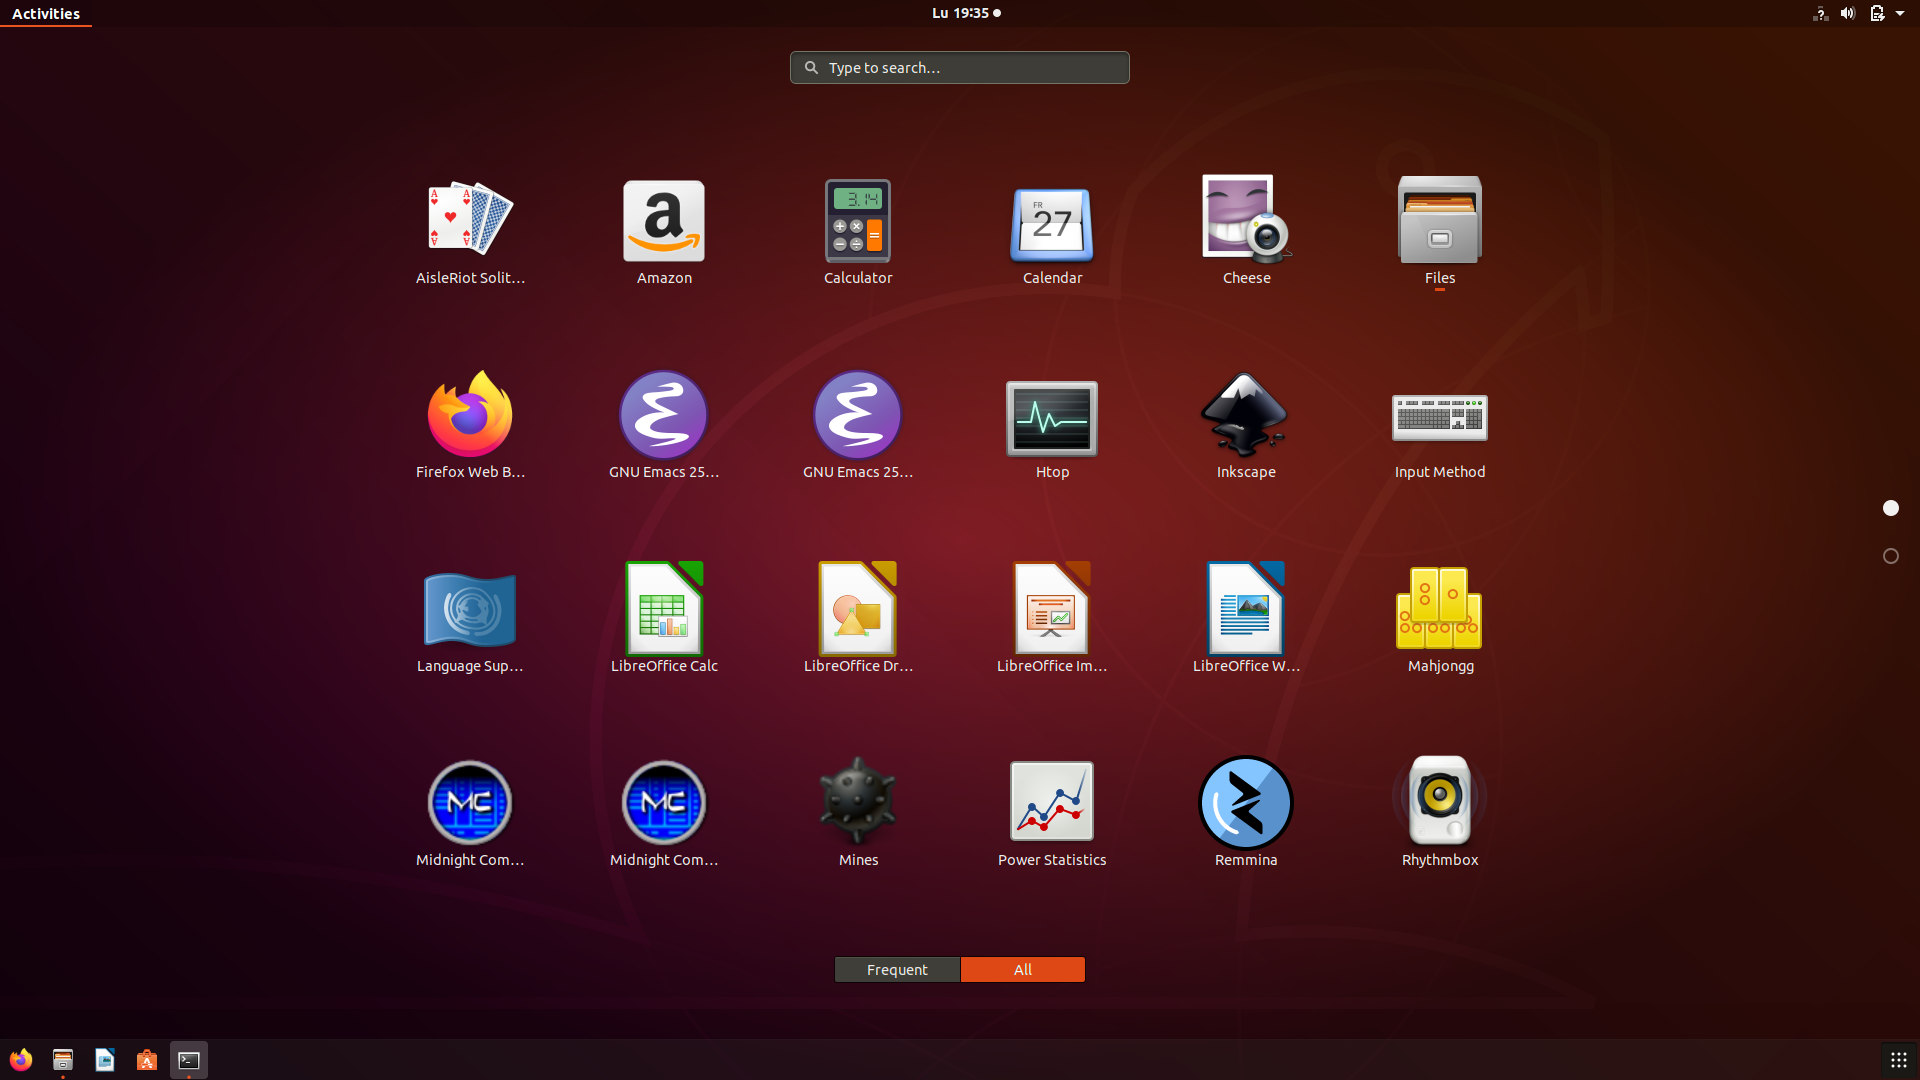
\includegraphics[width=\textwidth]{chapters/01-ui/img/gui-shell-screenshot.png}
    \caption{Shell GUI}
    \label{fig:ui:shell-gui-cli:gui}
  \end{subfigure}

  \begin{subfigure}[b]{0.6\textwidth}
    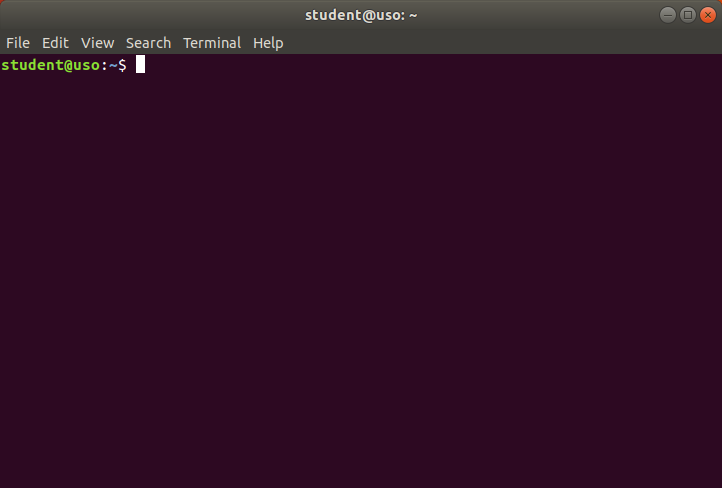
\includegraphics[width=\textwidth]{chapters/01-ui/img/cli-shell-screenshot.png}
    \caption{Shell CLI}
    \label{fig:ui:shell-gui-cli:cli}
  \end{subfigure}

  \caption{Shell GUI și CLI în Ubuntu 18.04}
  \label{fig:ui:shell-gui-cli}
\end{figure}

În capitolul curent ne vom concentra pe interfața grafică. Interfața în linia de comandă o vom discuta detaliat în \labelindexref{Capitolul}{chapter:cli}.

\section{Interfața grafică}
\label{sec:ui:gui}

Interfața grafică este comună pe majoritatea sistemelor desktop și este universală pe dispozitive mobile, dispozitive de tip smartwatch sau smart TV.

În mod clasic interfața grafică este compusă din elementele \textbf{WIMP}: \textit{Window}, \textit{Icon}, \textit{Menu}, \textit{Pointer}. Aceste elemente se regăsesc în interfețele cu ferestre comune sistemelor desktop. Pe sistemele mobile sau pe smart TV sau smartwatch, elementele sunt similare, cu diferența că, în mod uzual, nu sunt prezente mai multe ferestre simultan pe ecranul prezentat utilizatorului.

Pointerul din interfața grafică este controlat cu mouse-ul sau o telecomandă specifică sau este îndeplinit de deget pe ecranul tactil (\textit{touchscreen}) al dispozitivelor mobile. Cu ajutorul acestuia se activează (prin click) elemente din interfața grafică: iconuri, meniuri, butoane, sau se poate face \textit{drag and drop} sau alte acțiuni de aranjare a interfeței grafice.

Interfața grafică poate fi personalizată: scheme de culori, fonturi, dimensiuni, plasare elemente grafice pot fi modificate. Uzual noțiunea de ,,temă'' include o agregare de fonturi, culori și plasare a elementelor; un utilizator poate selecta între diferite teme pentru a alege interfața grafică potrivită. Această personalizare poate fi făcută atât pentru shellul sistemului de operare cât și pentru interfața grafică expusă de diferite aplicații. Adică pentru shellul sistemului de operare putem alege o dimensiune a iconurilor și o schemă de culori, în vreme ce pentru interfața unei aplicații precum Firefox (browser web) putem alege folosirea anumitor imagini pentru iconuri sau ascunderea anumitor meniuri.

Pentru accelerarea acțiunilor în interfața grafică, există în mod uzual scurtături de tastatură. Este o practică frecventă în lumea jocurilor de calculator (unde celebrele actions-per-minute (APM)) se bazează pe folosirea scurtăturilor din tastatură. În interfața în linia de comandă scurtăturilor sunt folosite pentru gestiunea ferestrelor, accesarea rapidă a unor elemente din meniuri.

În instalările implicite, sistemele de operare desktop oferă interfața grafică. Pentru tipurile de acțiuni care necesită interfața în linia de comandă (precum acțiuni mai specifice, sau acțiuni de automatizare sau acțiuni care nu se pot realiza altfel), se pot porni shelluri CLI din interfața grafică. Într-un mediu GNOME se poate porni o fereastră GNOME Terminal, în într-un mediu grafic Windows se poate porni o fereastră PowerShell. În \labelindexref{Figura}{fig:ui:shell-cli-linux-windows} sunt screenshot-uri cu două ferestre din mediul GUI în care rulează un shell CLI, una în Linux și alta în Windows. Este modul uzual în care rulăm comenzi în sistemele desktop moderne.

\begin{figure}[!htbp]
  \centering
  \begin{subfigure}[b]{0.6\textwidth}
    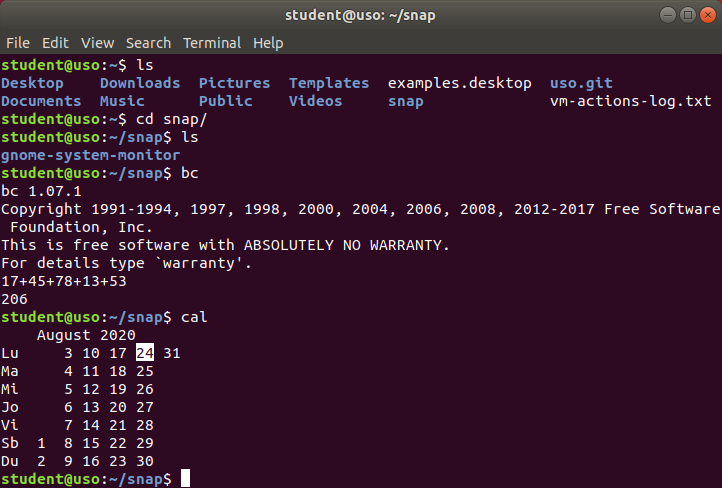
\includegraphics[width=\textwidth]{chapters/01-ui/img/linux-terminal.png}
    \caption{Linux}
    \label{fig:ui:shell-cli:linux}
  \end{subfigure}

  \begin{subfigure}[b]{0.6\textwidth}
    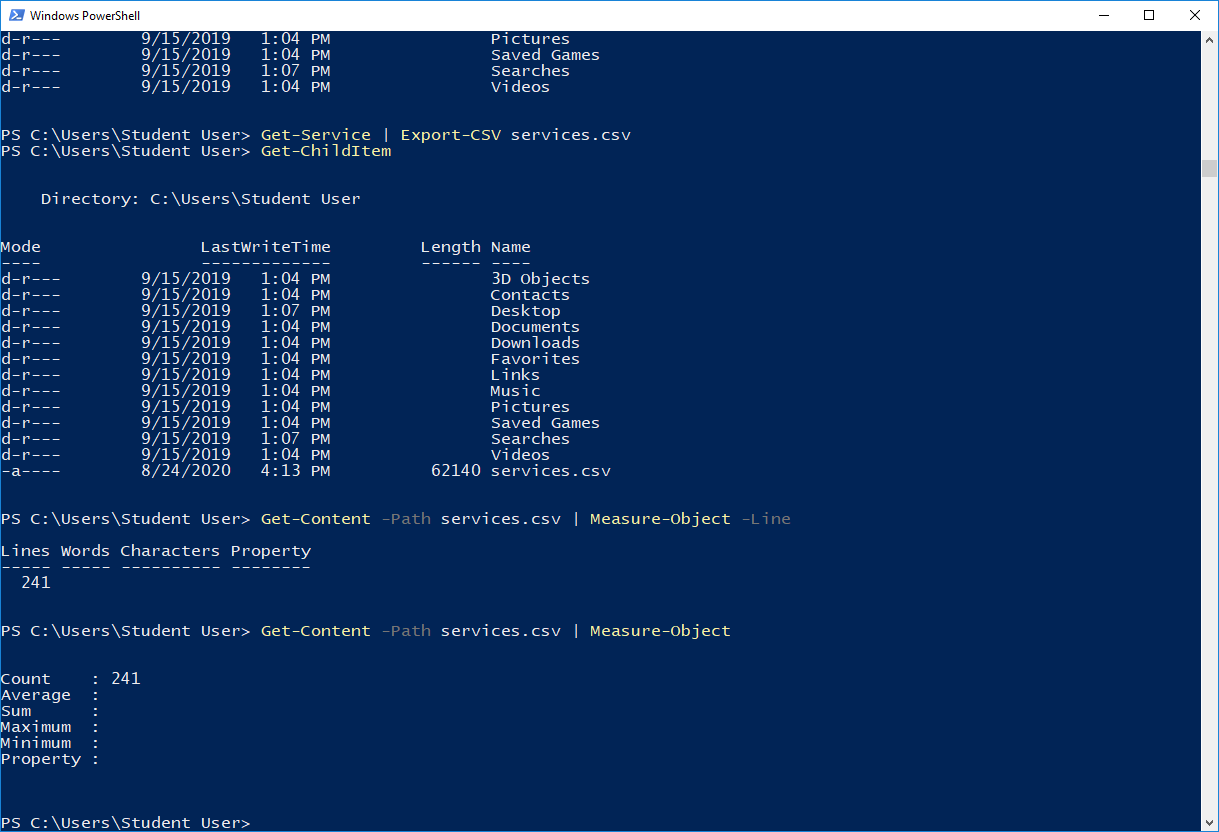
\includegraphics[width=\textwidth]{chapters/01-ui/img/powershell.png}
    \caption{Windows}
    \label{fig:ui:shell-cli:windows}
  \end{subfigure}

  \caption{Shell CLI (terminal) în Linux și în Windows}
  \label{fig:ui:shell-cli-linux-windows}
\end{figure}

\subsection{Interfețe native și interfețe web}
\label{sec:ui:native-web}

Interfețele web sunt tot forme de interfața grafică, folosind componente precum meniuri, iconuri, pointer, butoane. Spunem că o aplicație are interfață GUI dacă rulează de sine stătătoare pe un sistem de calcul; o numim \textbf{aplicație nativă}. Altfel, aplicațiile web oferă o interfață grafică web (numită și WebUI - \textit{web user interface}) în cadrul unui browser.

De avut în vedere că în ultimii ani asistăm la o migrare spre interfețe grafice web. Sistemele de operare desktop moderne oferă mai puține aplicații preinstalate, majoritatea elementele grafice (WIMP) fiind migrate în aplicații web. Adesea, un utilizator va porni un browser și din browser își va executa majoritatea acțiunilor: urmărit filme, ascultat muzică, lucrat la documente folosind suita Google Docs sau Office 360, comunicat online (Facebook Messenger, WhatsApp), publicat conținut (Facebook, Pinterest), inclusiv dezvoltat de aplicații.

Aplicațiile web sunt uzuale mediului desktop. În mod obișnuit, pe dispozitivele mobile sau de tip smart TV sau altele, aceste aplicații sunt aplicații native. În continuare pot fi accesate și prin browser, dar forma uzuală este cea de aplicație nativă. Adică pe un mediu desktop vom accesa din browser aplicația Facebook sau YouTube, pe când pe un dispozitiv mobil aceste aplicații sunt native; se poate accesa o aplicație web și pe un dispozitiv mobil prin intermediul unui browser, dar nu este o acțiune obișnuită pentru utilizator.

Motivul migrării aplicațiilor desktop în aplicații web este portabilitatea: dat fiind un browser (Mozilla Firefox, Google Chome sau altul), aplicațiile web se vor comporta la fel indiferent de sistemul de operare sau distribuția rulată. Altfel, este nevoie de o aplicație nativă pentru fiecare sistem de operare sau distribuție. În zona dispozitivele mobile sau smart TV, furnizorul dispozitivului oferă și sistemul de operare iar aplicațiile sunt create doar pentru acesta.

\subsection{Utilizabilitate și experiența utilizatorului}
\label{sec:ui:ux}

În proiectarea interfeței grafice este esențial ca aceasta să fie cât mai intuitivă și ușor de folosit. Noțiunea de experiența utilizatorului (\textit{user experience} - UX) este centrală pentru aplicațiile și dispozitivele cu interfața grafică. O interfața încărcată, cu elemente greu accesibile sau neintuitiv plasate va fi respinsă de utilizator care va alege altă aplicație sau altă platformă.

Organizațiile care dezvoltă interfețe grafice stabilesc principii și recomandări de urmat. Acest principii țin cont de natura umană și comportamentul utilizatorilor, în general din studii specifice, și se regăsesc în documente numite \textit{Human Interface Guidelines} (Ghiduri de interfațare om-calculator). Exemple de organizații și astfel de documente sunt:

\begin{itemize}
  \item GNOME: \textit{GNOME Human Interface Guidelines}\footnote{\url{https://developer.gnome.org/hig/stable/}}
  \item Apple: \textit{Apple Human Interface Guidelines}\footnote{\url{https://developer.apple.com/design/human-interface-guidelines/}}
  \item Android: \textit{Android Design Guidelines}\footnote{\url{https://developer.android.com/design}}
  \item Microsoft: \textit{Microsoft User Interface Principles}\footnote{\url{https://docs.microsoft.com/en-us/windows/win32/appuistart/-user-interface-principles}}
\end{itemize}

O aplicație sau un dispozitiv de succes va trebuie să țină cont și de interfața grafică, nu numai de funcționalitățile și performanța sa. Aspectele ce țin de experiența utilizatorului sunt cu atât mai importante pe dispozitivele mobile unde interfața grafică tactilă este universală. În aceeași măsură, aplicațiile și site-urile web necesită interfețe intuitive pentru satisfacția utilizatorilor acestora. Un utilizator nemulțumit sau încurcat de interfață nu va folosi aplicația, lucru care se traduce în general în pierderi financiare. De aceea, aspectele ce țin de experiența utilizatorului sunt esențiale pentru dezvoltatorii de aplicații pe dispozitive mobile sau aplicații web.

\section{Interfața grafică în Linux}
\label{sec:ui:linux-gui}

Așa cum am precizat și în \labelindexref{Capitolul}{chapter:intro}, Linux (sau mai bine spus, distribuțiile software bazate pe Linux) rulează pe o plajă largă de sisteme și dispozitive: server, desktop/laptop, mobile (Android), smart TV, smart watch, rutere/echipamente de rețea etc. Fiecare dintre aceste sisteme oferă o interfață utilizatorului:

\begin{itemize}
  \item interfață grafică tactilă, în cazul dispozitivelor mobile sau smart watch
  \item interfață grafică și telecomandă, în cazul smart TV
  \item interfață în linie de comandă sau interfață web de configurare, în cazul echipamentelor de rețea
  \item interfață în linie de comandă, în cazul serverelor
  \item interfață grafică și în linie de comandă, în cazul sistemelor desktop/laptop
\end{itemize}

În cele ce urmează vom prezenta interfața grafică în cazul sistemelor desktop/laptop. Deși nu este obișnuit, această interfață poate fi prezentă și în cazul sistemelor server. Interfața în linia de comandă va fi prezentată în formă de comenzi Linux în restul capitolelor și detaliat în \labelindexref{Capitolul}{chapter:cli}.

\subsection{Desktop Environments}
\label{sec:ui:desktop-environments}

Suita de componente software care oferă interfața grafică utilizatorului într-un sistem de operare formează un mediu desktop (\textit{desktop environment}), așa numitul shell GUI. Putem spune că toate sistemele de operare oferă un desktop environment pe majoritatea tipurilor de dispozitive. Termenul a fost însă popularizat și este folosit cu precădere în sistemele de operare din lumea Unix/Linux.

În lumea Linux posibilitatea de personalizare a distribuțiilor software este foarte mare, inclusiv a mediului desktop folosit. O distribuție Linux oferă o configurație implicită de mediu desktop, care poate fi însă modificată.

Alegerea unui mediu desktop ține de consumul de resurse, de posibilitățile de personalizare și preferința și istoricul utilizatorului. Un mediu desktop oferă un anume aspect, o selecție și configurare a componentelor software, și aplicații specifice pentru acțiuni uzuale (navigare în sistemul de fișiere, navigare web, redare multimedia, editor text, emulator de terminal).

Exemple de medii desktop în Linux sunt GNOME, KDE, MATE, Cinnamon, Budgie, Xfce. O comparație a acestora și referințe la articole comparative se găsește pe Wikipedia\footnote{\url{https://en.wikipedia.org/wiki/Comparison\_of\_X\_Window\_System\_desktop\_environments}}. Aplicațiile grafice de bază (precum browerul în sistemul de fișiere, editor text, player multimedia) sunt parte a fiecărui mediu desktop, fiecare mediu cu particularitățile sale. Alte aplicații grafice sunt instalate, majoritatea nefiind specifice unui mediu desktop; de exemplu, Mozilla Firefox este un browser web iar VLC este un player multimedia care nu sunt specifice unei anumite distribuții.

\subsection{Sistemul de ferestre (Window System)}
\label{sec:ui:window-system}

Redarea elementelor grafice ale unei aplicații ce rulează peste sistemul de operare este gestionată de sistemul de ferestre. Sistemul de ferestre este un ansamblu software care interacționează cu sistemul de operare, componente ale mediului desktop și cu aplicațiile. Fiecare sistem de operare (nu doar Linux) are un sistem de ferestre. În Windows, este reprezentat de Desktop Windows Manager; în macOS, este reprezentat de Quartz și Core Graphics.

Sistemul de ferestre este compus în mod uzual din:

\begin{itemize}
  \item manager de ferestre/afișare (\textit{window/display manager}): gestionează așezarea ferestrelor pe ecran, uzual încluzând bare de meniuri.
  \item widget/GUI toolkit: colecție de biblioteci care oferă elementele grafice (numite widgeturi), folosit de managerul de ferestre.
  \item server de ferestre/afișare (\textit{window/display server}): interacționează printr-un protocol specific cu aplicațiile grafice, cu sistemul de operare și cu managerul de ferestre pentru redarea componentelor grafice.
\end{itemize}

Schematic, componentele sistemului de ferestre sunt indicate în \labelindexref{Figura}{fig:ui:window-system}\footnote{\url{https://commons.wikimedia.org/wiki/File:Schema_of_the_layers_of_the_graphical_user_interface.svg} (CC BY-SA 3.0)}.

\begin{figure}[htbp]
  \centering
  \def\svgwidth{\columnwidth}
  \includesvg{chapters/01-ui/img/window-system.svg}
  \caption{Componentele sistemului de ferestre}
  \label{fig:ui:window-system}
\end{figure}

Delimitarea între componentele sistemului de ferestre din \labelindexref{Figura}{fig:ui:window-system} nu este strictă, mai ales în sistemele de operare diferite de Linux.

În mod implicit, managerii de ferestre folosiți implicit pe majoritatea distribuțiilor Linux sunt flotanți (\textit{floating/stacking window manager}). Adică ferestrele pot fi suprapuse și mișcate în funcție de preferințele utilizatorilor. Un alt tip de manager de ferestre este cel bazat pe secțiuni (\textit{tiling window manager}); în acest caz fiecare fereastră ocupă un spațiu fix în ecran, fără a se suprapune cu alte ferestre; ecranul este secționat cu ferestre diferite ocupând un spațiu nesupraspus cu altele. Exemple de tiling window managers sunt i3\footnote{\url{https://i3wm.org/}}, awesome\footnote{https://awesomewm.org/}, bspwm\footnote{https://github.com/baskerville/bspwm}. Unii manageri sunt dinamici permițând tranziția între modul floating și modul tiling.

În Linux, în mod tradițional, sistemul de ferestre folosit este X Window System\footnote{\url{https://www.x.org/wiki/}}, sau, mai simplu, X. În ultima perioadă a căpătat tracțiune alternativa Weyland/Weston\footnote{\url{https://wayland.freedesktop.org/}}, apărută ca reacție la complexitatea X. Weyland/Weston se dorește a fi o soluție mai simplă și cu proiectare mai sigură. Weyland/Weston nu este încă adoptat pe scară largă, astfel că multe distribuții sau medii desktop preferă folosirea X, care este mai stabil.

Aspectul comun al X și Weyland este interacțiunea componentelor. X și Weyland sunt de fapt specificații de protocoale și implementări de referință ale acestora pentru interacțiunea între serverul de ferestre (window server) și aplicațiile grafice (clienți grafici).

Schema de funcționare a X/Weyland este prezentată în \labelindexref{Figura}{fig:ui:x-window-system}\footnote{\url{https://commons.wikimedia.org/wiki/File:X_client_server_example.svg} (CC BY-SA 3.0)}

\begin{figure}[htbp]
  \centering
  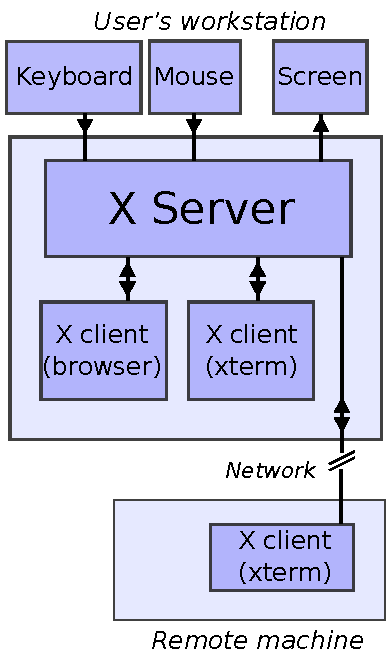
\includegraphics[width=0.3\textwidth]{chapters/01-ui/img/x-window-system.pdf}
  \caption{Funcționarea sistemului de ferestre în Linux (X sau Weyland)}
  \label{fig:ui:x-window-system}
\end{figure}

În interacțiunea indicată în \labelindexref{Figura}{fig:ui:x-window-system}, o aplicație precum Mozilla Firefox este client grafic (\textit{X client} în figură). Folosind protocolul X/Weyland, aplicația transmite către serverul X/Weyland (\textit{X server} în figură) cerințele sale de afișare grafică pe ecran (\textit{Screen} în figură). Aceste cerințe sunt rezultate de obicei din acțiunile utilizatorului, cu ajutorul mouse-ului sau tastaturii (\textit{Keyboard} și \textit{Mouse} în figură) sau a altor dispozitive. Aceste acțiuni ajung la aplicație ștot prin intermediul serverului X. Practic, aplicația client se ocupă de resursele sale de calcul lăsând serverului grafic responsabilitatea interacțiunii cu utilizatorul.

Una dintre funcționalitățile X, absentă din Weyland, este folosirea peste rețea, indicată în \labelindexref{Figura}{fig:ui:x-window-system} (\textit{Network}). În această situație, aplicația client rulează pe un sistem la distanță (\textit{Remote machine} în figură), iar serverul X rulează pe sistemul local (\textit{User's workstation} în figură). Interacțiunea între aplicația client și aplicația server are loc prin rețea prin intermediul protocolului X. Practic, pașii urmați sunt:
\begin{enumerate}
  \item Utilizatorul folosește echipamentele locale (mouse, tastatură) pentru a executa acțiuni.
  \item Acțiunile utilizatorului sunt capturate de serverul X local.
  \item Serverul X local transmite aceste transmise de server prin rețea către aplicația client ce rulează la distanță.
  \item Aplicația client execută aceste acțiuni și generează un rezultat care să fie afișat (pixeli, culori, ferestre etc.)
  \item Rezultatul este transmis de aplicația client prin rețea către serverul X.
  \item Serverul X redă rezultatul pe afișajul local.
  \item Utilizatorul vede pe afișajul local rezultatul acțiunilor sale inițiale.
\end{enumerate}

În secvența de mai sus, întrucât aplicația client rulează pe sistemul de la distanță, consumul de resurse (procesor, memorie, sistem de fișiere) se face pe acel sistem. Sistemul local (pe care rulează serverul X) ocupă resurse doar pentru interacțiune cu utilizatorul (ecran, tastatură, mouse).

Aplicații grafice pot fi rulate la distanță și dacă sistemul local rulează Windows sau macOS. Pentru aceasta este nevoie de instalarea unui server X nativ Windows, precum XMing\footnote{\url{https://sourceforge.net/projects/xming/}}, sau a unui server nativ macOS, precum XQuartz\footnote{\url{https://www.xquartz.org/}}.

În mod uzual, din rațiuni de securitate, rularea la distanță de aplicații X grafice se realizează peste un canal SSH, protocol despre care vom discuta în \labelindexref{Secțiunea}{sec:sec:ssh}.

\subsection{Funcționalități ale interfeței grafice în Linux}
\label{sec:ui:linux-gui-features}

Pe lângă elementele grafice de tipul WIMP, interfața grafică în Linux oferă utilizatorilor și alte funcționalități.

O astfel de funcționalitate este prezența de de spații de lucru (\textit{workspace}) multiple, sau desktopuri multiple. Într-o sesiune de mediu grafic pot exista mai multe workspace-uri/desktopuri, fiecare cu ferestrele sale; utilizatorul poate migra între workspace-uri pentru a compartimenta aplicațiile și ferestrele în funcție de nevoi. Depinzând de mediul desktop, numărul de workspace-uri este static (fixat într-o configurație) sau dinamic (se poate crea rapid un workspace nou). În oricare situație, acțiunile sunt: tranziție la un alt workspace sau mutare fereastră într-un alt workspace. O funcționalitate similară este prezentă în macOS, numită Mission Control, și în Windows, de la Windows 10.

Pentru a executa acțiuni rapide în mediul grafic sunt utile scurtăture de tastatură (\textit{keyboard shortcuts}). În general, orice mediu grafic oferă scurtături pentru pornire de aplicații, închidere de aplicații, deschidere și închidere de tab-uri de aplicație, minimizat ferestre, accesat meniuri, schimbat între ferestre. Aceste scurtături depind de sistemul de operare și mediul desktop folosit. O listă a scurtăturilor folosite pe mașina virtuală de suport a acestei cărți (Ubuntu 18.04) este în \labelindexref{Tabelul}{tab:ui:vm-shortcuts}.

O parte dintre acțiunile utilizatorului pot fi realizate doar sau mai rapid în interfața în linia de comandă. Pentru acesta, din mediul grafic se pot porni rapid aplicații shell în linia de comandă, în forma emulatoarelor de terminal \textit{terminal emulator}. Un emulator de terminal este o aplicație care prezintă utilizatorului o fereastră. În această fereastră rulează un shell CLI unde utilizatorul poate rula comenzi. De exemplu, în \labelindexref{Figura}{fig:ui:shell-cli-linux-windows}, prima imagine este o fereastră de emulator de terminal în GNOME (aplicația \texttt{gnome-terminal}) în care rulează shellul Bash; în mod similar, cealaltă imagine este o fereastră Windows în care rulează shellul PowerShell. În macOS acest rol în are aplicația Terminal, care este preinstalată în sistemul de operare. Sunt și alte emulatoare de terminal care pot fi instalate în locul sau pe lângă cele implicite. Mai multe informații despre terminale, emulatoare de terminal și shell vom prezenta în \labelindexref{Capitolul}{chapter:cli}.

\section{Interfața grafică în mașina virtuală de suport}
\label{sec:ui:vm}

Distribuțiile, mediile desktop, managerii de ferestre și aplicațiile Linux sunt diverse. Este dificil de găsit un numitor comun de aspecte generice, comune tuturor. În această secțiune vom prezenta informații specifice mașinii virtuale de suport a cărții, mașină care rulează Ubuntu 18.04.

Așa cum am precizat mai sus, pentru acțiuni rapide în interfața grafică a unui sistem de operare (și, în general, a unei aplicații) sunt utile scurtăturile de tastatură. \labelindexref{Tabelul}{tab:ui:vm-shortcuts} conține cele mai comune scurtături în mașina virtuală.

\begin{table}[!htb]
  \caption{Scurtături de tastatură în mașina virtuală de suport}
  {\scriptsize
  \begin{center}
    \begin{tabular}{ p{0.22\textwidth} p{0.3\textwidth} p{0.38\textwidth} }
      \toprule
        \textbf{Scurtătură} &
        \textbf{Efect} &
        \textbf{Aplicații în care are efect} \\
      \midrule
        \texttt{Alt+F2} &
        deschiderea promptului de rulare comenzi &
        în mediul grafic (nu într-o anume aplicație) \\
        %\addlinespace[5pt]
        \midrule

        \texttt{Alt+Ctrl+t} &
        deschiderea unui emulator de terminal &
        în mediul grafic (nu într-o anume aplicație) \\
        %\addlinespace[5pt]
        \midrule

        \texttt{Ctrl+n} &
        deschiderea unei aplicații identice &
        în majoritatea aplicațiilor grafice \\
        %\addlinespace[5pt]
        \midrule

        \texttt{Ctrl+t} &
        deschiderea unui nou tab &
        în aplicații cu taburi (browser web, browser de fișiere) \\
        %\addlinespace[5pt]
        \midrule

        \texttt{Ctrl+Shift+t} &
        deschiderea unui nou tab &
        în emulatorul de terminal \\
        %\addlinespace[5pt]
        \midrule

        \texttt{Ctrl+w} &
        închiderea unui tab (sau a ultimei ferestre) &
        în aplicații cu taburi (browser web, browser de fișiere, terminal) \\
        %\addlinespace[5pt]
        \midrule

        \texttt{Alt+1, Alt+2, \ldots} &
        nagivarea între taburi &
        în aplicații cu taburi (browser web, browser de fișiere, terminal) \\
        %\addlinespace[5pt]
        \midrule

        \texttt{Alt+Tab} &
        nagivarea între adrese &
        în mediul grafic (nu într-o anume aplicație) \\
        %\addlinespace[5pt]
        \midrule

        \texttt{Ctrl+l} &
        accesarea barei de adrese &
        în aplicații cu bare de adrese (browser web, browser de fișiere) \\
        %\addlinespace[5pt]
        \midrule

        \texttt{Alt+F4} &
        închiderea unei ferestre de aplicație &
        în toate aplicațiile \\
        %\addlinespace[5pt]
        \midrule

        \texttt{Alt+Ctrl+d} &
        afișarea desktopului (cu minimizarea tuturor ferestrelor) &
        în mediul grafic (nu într-o anume aplicație) \\
        %\addlinespace[5pt]
        \midrule

        \texttt{Alt+F10} &
        maximizare / minimizare aplicații (comutare) &
        în toate aplicațiile \\
        %\addlinespace[5pt]
        \midrule

        \texttt{Alt+Ctrl+săgeți} &
        navigarea între workspace-uri &
        în mediul grafic (nu într-o anume aplicație) \\
        %\addlinespace[5pt]
        \midrule

        \texttt{Alt+Ctrl+l} &
        închidere ecran (\textit{lock screen}) &
        în mediul grafic (nu într-o anume aplicație) \\
        %\addlinespace[5pt]

      \bottomrule
    \end{tabular}
    \label{tab:ui:vm-shortcuts}
  \end{center}
  }
\end{table}

O scurtătură frecventă de tastatură, întâlnită pe majoritatea distribuțiilor și mediilor desktop, este \texttt{Alt+F2} folosită pentru pornirea rapidă a unei aplicații, introducând numele comenzii, la fel ca în \labelindexref{Figura}{fig:ui:app-launcher}. Funcționalitatea este numită \textit{application launcher}. Echivalentul în Windows este \texttt{Windows+r}, iar în macOS \texttt{Command+Space}.

\begin{figure}[!htbp]
  \centering
  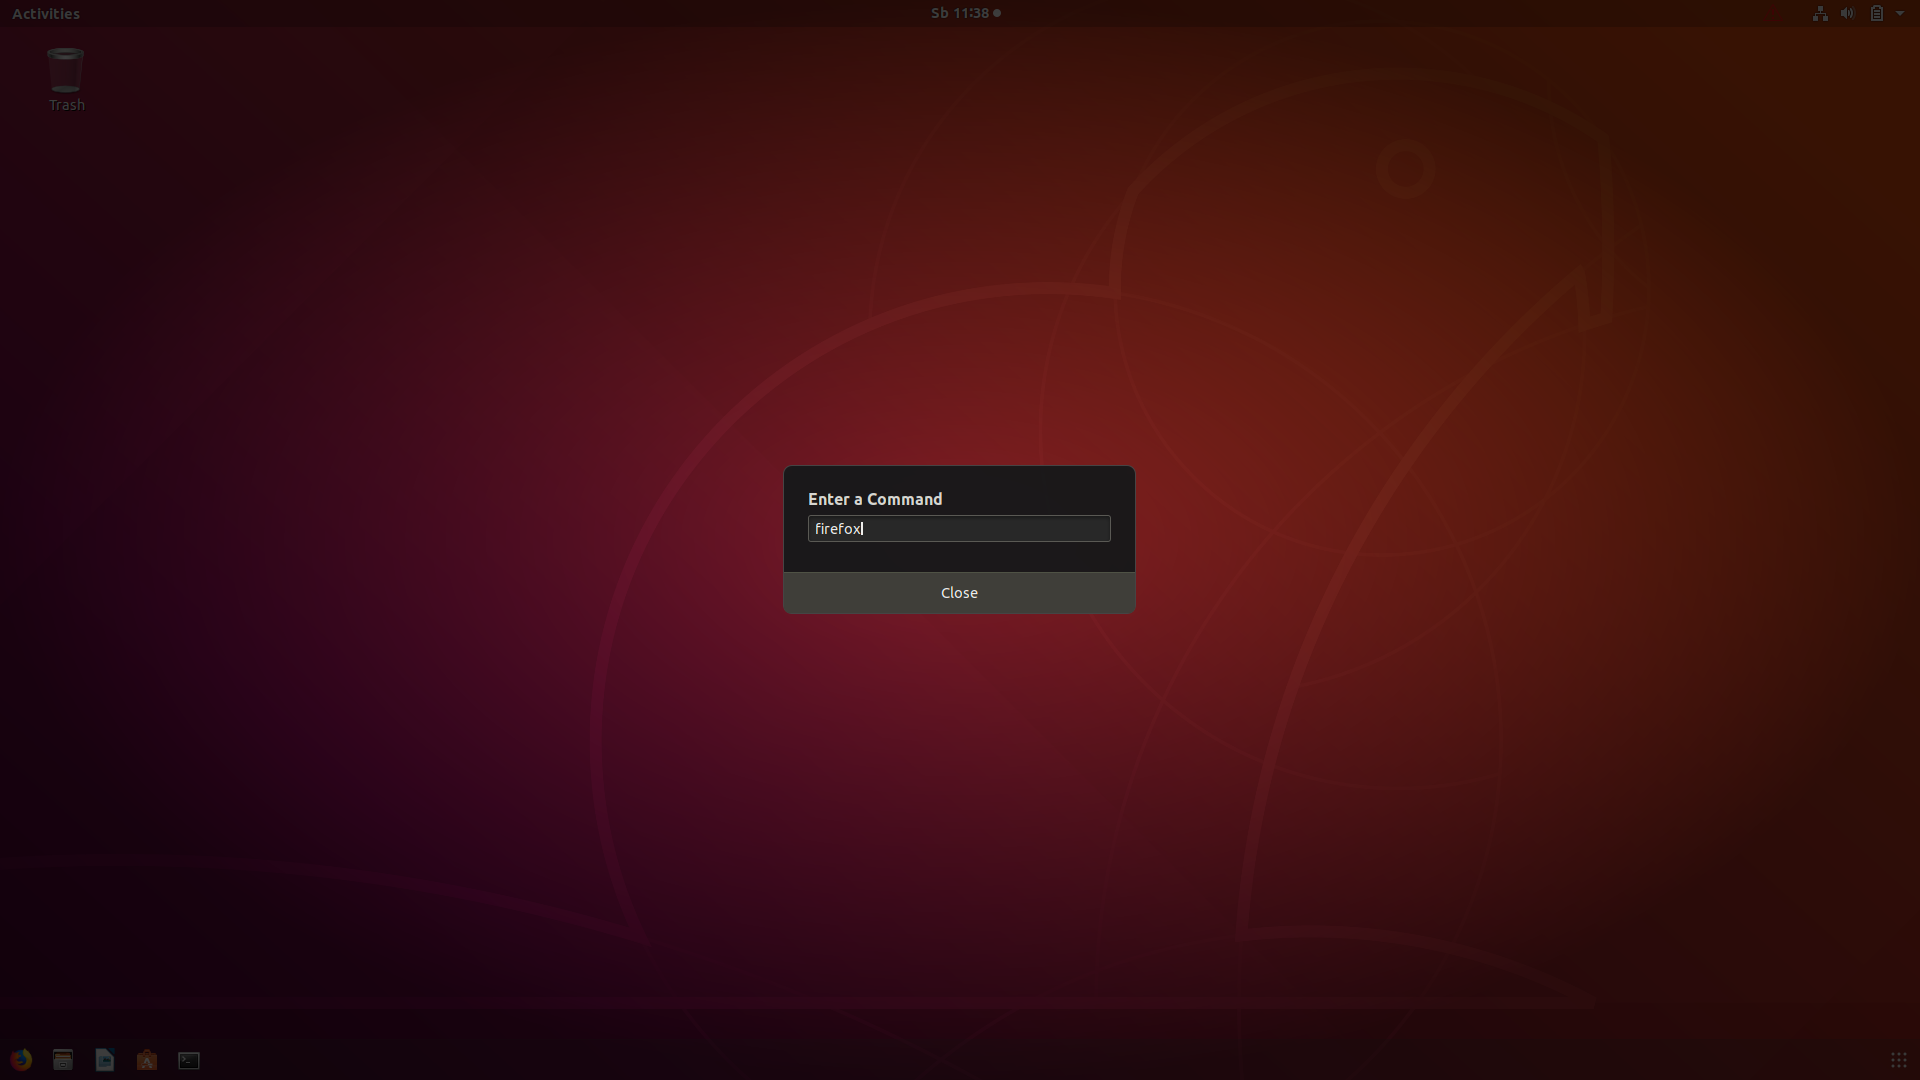
\includegraphics[width=0.6\textwidth]{chapters/01-ui/img/alt+f2.png}
  \caption{Rularea unei aplicații din mediul grafic în Linux (\textit{application launcher})}
  \label{fig:ui:app-launcher}
\end{figure}

Sunt mai multe scurtături de tastatură, majoritatea fiind configurabile. Pentru vizualizarea și, eventual, configurarea acestora în mașina virtuală se accesează \texttt{System Settings $\rightarrow$ Devices $\rightarrow$ Keyboard}; va rezulta un ecran precum cel din \labelindexref{Figura}{fig:ui:keyboard-shortcuts}. Aplicația \textit{System Settings} se accesează din interfața grafică sau prin rularea comenzii \texttt{gnome-control-center}.

\begin{figure}[!htbp]
  \centering
  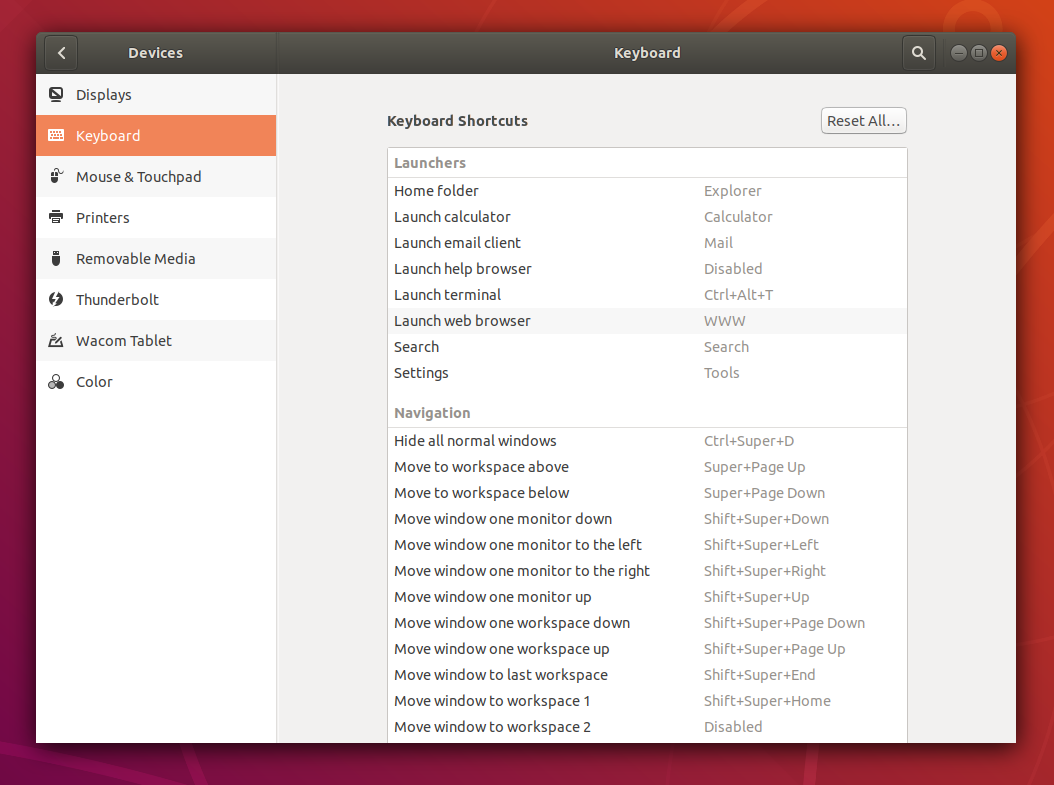
\includegraphics[width=0.6\textwidth]{chapters/01-ui/img/keyboard-shortcuts.png}
  \caption{Vizualizarea și configurarea scurtăturilor de tastatură}
  \label{fig:ui:keyboard-shortcuts}
\end{figure}

O acțiune frecventă la instalarea sistemului de calcul este configurarea schemei de tastatură (\textit{keyboard layout}). Dacă dorim adăugarea unei noi scheme de tastatură, acest lucru se face prin accesarea meniului de tastatură din pașii \texttt{System Settings $\rightarrow$ Region \& Language}. Vom ajunge la un ecran precum cel din \labelindexref{Figura}{fig:ui:keyboard-layout}, unde putem configura noi scheme de tastatură.

\begin{figure}[!htbp]
  \centering
  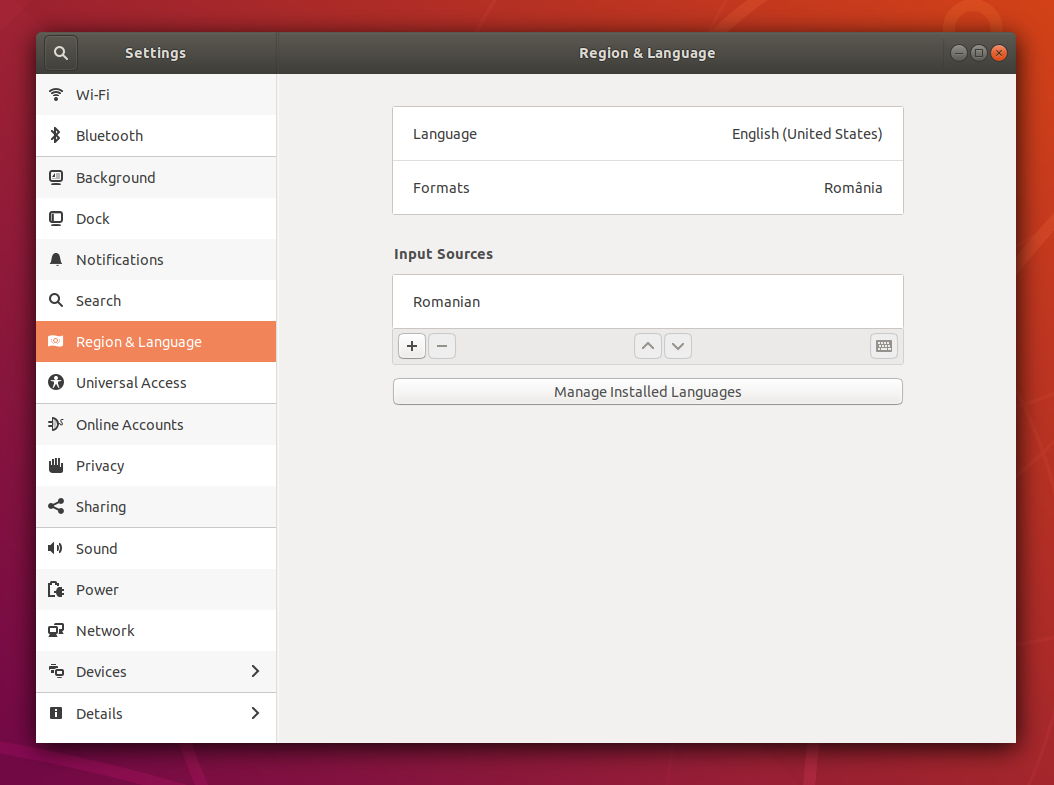
\includegraphics[width=0.6\textwidth]{chapters/01-ui/img/keyboard-layout.png}
  \caption{Configurarea schemei de tastatură (keyboard layout)}
  \label{fig:ui:keyboard-layout}
\end{figure}

În general configurațiile se pot realiza din meniurile aplicațiilor sau din aplicația \textit{System Settings} (pornită din interfața grafică sau cu ajutorul comenzii \texttt{gnome-control-center}. Anumite configurații (precum dezactivarea introducerii parolei la autentificare) necesită accesarea interfeței de configurare. Pentru aceasta folosim comandda \texttt{dconf-editor} pentru a porni aplicația \textit{Dconf Editor}, la fel ca în \labelindexref{Figura}{fig:ui:dconf-editor}, cu care avem acces la o plajă largă de opțiuni de configurare.

\begin{figure}[!htbp]
  \centering
  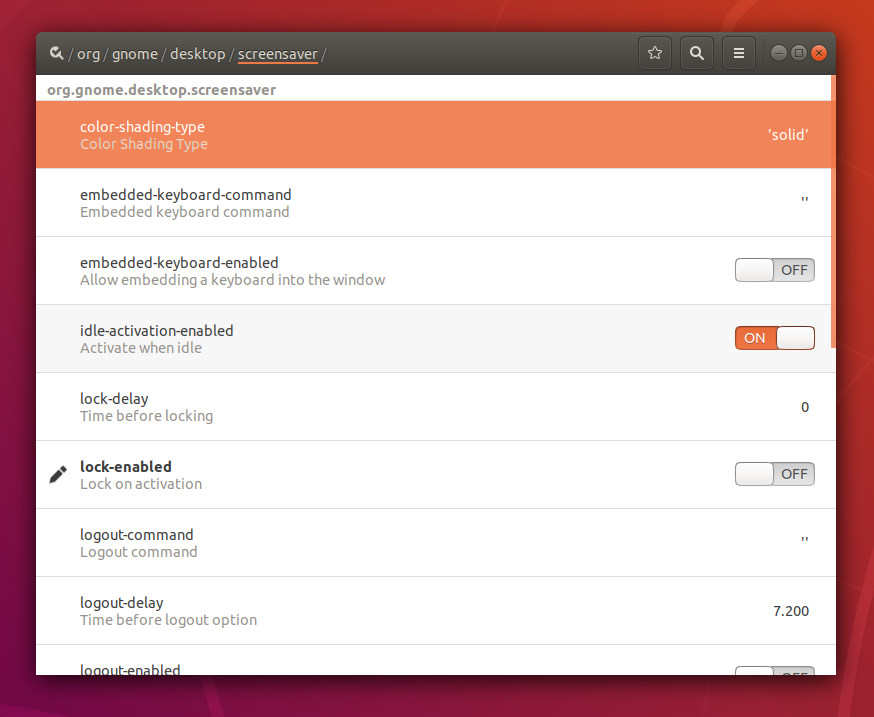
\includegraphics[width=0.6\textwidth]{chapters/01-ui/img/dconf-editor.png}
  \caption{Opțiuni de configurare în mediul grafic (dconf-editor)}
  \label{fig:ui:dconf-editor}
\end{figure}

În mod implicit, în Linux, desktopul conține puține scurtături de desktop (\textit{desktop shortcuts}) sau alte iconuri. Aceasta pentru că aplicațiile pot fi pornite rapid folosit scurtătura de tip \textit{application launcher} (\texttt{Alt+F2}). Dacă însă dorim să creăm o scurtătură de desktop, putem face acest fie creând manual un fișier cu extensia \texttt{.desktop}\footnote{\url{https://linuxconfig.org/how-to-create-custom-desktop-files-for-launchers-on-linux}} sau folosind comanda \texttt{gnome-desktop-item-edit}, ca mai jos:

\begin{screen}
student@uso:~$ gnome-desktop-item-edit ~/Desktop/Skype.desktop
\end{screen}

La rularea acestei comenzi, va apărea o fereastră precum cea din \labelindexref{Figura}{fig:ui:desktop-shortcut} unde vom introduce informațiile legate de aplicația Skype pentru care dorim crearea scurtăturii: calea către executabil, numele, iconul. În final va fi creat fișierul \texttt{Skype.desktop} care va apărea pe desktop și cu care vom putea porni, ca scurtătură de desktop, aplicația Skype.

\begin{figure}[!htbp]
  \centering
  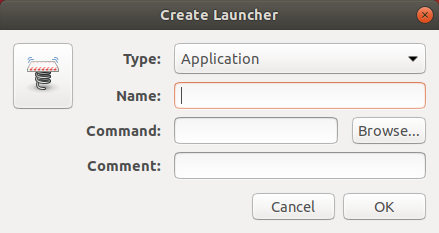
\includegraphics[width=0.4\textwidth]{chapters/01-ui/img/desktop-shortcut.png}
  \caption{Configurarea unei scurtături de desktop}
  \label{fig:ui:desktop-shortcut}
\end{figure}

\section{Sumar}
\label{sec:ui:summary}

Sistemul de operare oferă o interfață (shell) pentru interacțiunea utilizatorului cu aplicațiile și sistemul de operare.

Shell-ul poate fi grafic (GUI) sau în linia de comandă. Shellul grafic este mai intuitiv și preferat majorității utilizatorilor. Interfața în linia de comandă permite acces la un spațiu mai mare de opțiuni și acțiuni și posibilitatea automatizării prin scripturi.

Interfața grafică este compusă din elemente grafice acționate cu mouse-ul sau tactil, sub acronimul WIMP (\textit{Window, Icon, Menu, Pointer}).

Interfața grafică trebuie să fie simplă și intuitivă. Aplicațiile și sistemele de operare urmăresc recomandări de proiectare a interfeței pentru a oferi o experiență bună utilizatorului.

În Linux interfața grafică vine în formă de mediu desktop (\textit{desktop environment}), o suită software cu shell grafic, aplicații grafice și opțiuni de configurare specifice. Exemple sunt GNOME și KDE.

Mediul grafic se bazează pe un sistem de ferestre. În Linux, în mod tradițional este folosit sistemul de ferestre X. În ultimi ani, a prins tracțiune sistemul de ferestre Weyland/Weston.

Mașina virtuală de suport a acestei cărți folosește un sistem de operare Ubuntu 18.04 cu interfață grafică GNOME.
